\chapter{Background}

\label{ch:background}
% \todo[inline, backgroundcolor=kth-lightblue]{Bakgrund}

% \todo[inline]{When you do your literature study, you should have a nearly complete Chapters 1 and 2.\\
% You may also find it convenient to introduce the future work section into your report early – so that you can put things that you think about but decide not to do now into this section.\\
% Note that later you can move things between this future work section and what you have done as you may change your mind about what to do now versus what to put off to future work.
% }
% \todo[inline]{What does a reader (another x student -- where x is your study line) need to know to understand your report?
% What have others already done? (This is the “related work”.) Explain what and
% how prior work / prior research will be applied on or used in the degree
% project /work (described in this thesis). Explain why and what is not used in
% the degree project and give valid reasons for rejecting the work/research.}

% This chapter provides basic background information about xxx. Additionally, this chapter describes xxx. The chapter also describes related work xxxx.



% \todo[inline, backgroundcolor=kth-lightblue]{Vilken viktig litteratur och
  % (forsknings-)artiklar har du studerat inom området (litteraturstudie)? }

% TODO: Introduce chapter

\section{Filesystems}
Filesystems are used to store data on for instance a hard drive of a computer on in the cloud. Google Drive is a filesystem that enables user to save their data online up to 15 GB for free\cite{CloudStorageWork} using their clusters of distributed storage devices, meaning that the data is saved on theirs servers which can be located wherever\cite{DistributedStorageWhat}. Paying customers can achieve higher amount of storage using the service.

A deniable filesystem is a system that does not expose files stored on this system without credentials - neither how many files are stored, their sizes, their content or even if there exists any files on the filesystem\cite{petersDEFYDeniableFile2014}. This is useful if for example one is to be exposed to an audit of their data by a totalitarian regim where they don't even want to disclose that they have data.

A unix filesystem uses a data structure called an \textit{inode}. An inode keeps track of the metadata for the files in the filesystem, and a directory simply contains the file names, and each files/directory's inode id. Using a lookup, the system can then learn about the file - where it is located, for instance how big it is, as can be seen in Figure~\ref{fig:inode_diag} (\textbf{CITATION NEEDED}). Each inode entry can contain any number of metadata information which might be relevant for the system, such as creation time and last updated.

\begin{figure}[!ht]
	\begin{center}
	  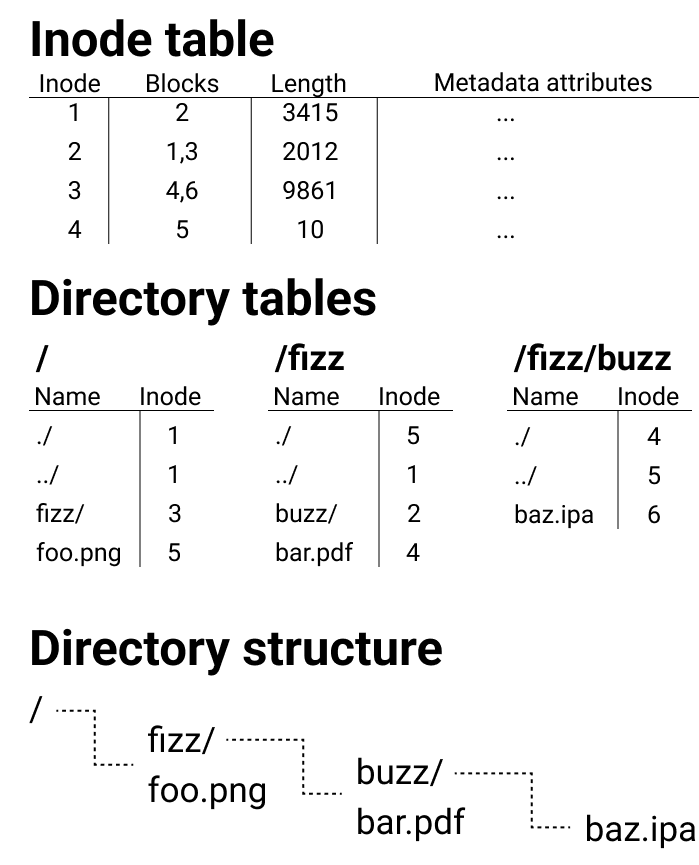
\includegraphics[width=0.8\textwidth]{figures/inode_diagram.png}
	\end{center}
	\caption{Basic structure of inode based filesystem}
	\label{fig:inode_diag}
\end{figure}

Looking at the 4 main file systems of windows, they all have many, sometimes different, functionalities such as links and named streams as well limitations such as a defined theoretical maximum file size\cite{mikbenFileSystemFunctionality}. This is set to 16 exbibytes for NTFS, exFAT and UDF, and for FAT32 it is set to 4 gigabytes. 

\section{Twitter}
\label{sec:twitter}
Twitter is a micro-blog online where users can sign up for a free account and create public posts (tweets) using text, images, and videos. Each post has a unique id associated with it\,\cite{twitterTwitterIDs}. Text posts are limited to $280$ characters while images can be up to \SI{5}{\mega\byte} and videos up to \SI{512}{\mega\byte}\,\cite{MediaBestPractices}. An post with images can contain up to 4 images in one post. There is also a possibility to send private messages to other accounts, where each message can contain up to $10\,000$ characters and the same limitations on files. However, direct messages older than $30$ days are not possible to retrieve through Twitter's API\,\cite{RetrievingOlder302018}. It is possible to create threads of Twitter posts where multiple tweets can be associated in chronological order.

Twitter's API defines technical limits of how many times certain actions can be executed by a user\,\cite{UnderstandingTwitterLimits}. A maximum of $2\,400$ tweets can be sent per day, and the limit is further broken down into smaller limits at semi-hourly intervals. Hitting a limit means that the user account no longer can perform the actions that the limit represents until the time period has elapsed.

\section{Threats}
To consider a filesystem secure it is important to imagine different potential adversaries who might attack the system. Considering that FFS has no real control of the data stored on the different services, all the data must be considered to be stored in an insecure system. Even if we could hide the posts made on for instance Twitter by making the profile private, we must still consider that Twitter themselves could be an adversary or that they could potentially give out information, such as tweets or direct messages, to entities such as the police. In fact, Twitter's privacy policy mentions that they may share, disclose, and preserve personal information and content posted on the service, even after account deletion for up to $18$ months\,\cite{TwitterPrivacyPolicy}. Therefore, to achieve security the data stored must always be encrypted. We assume that an adversary has access to all knowledge about FFS, including how the data is converted, encrypted, and posted. We also assume they know which websites and accounts that could post data from the filesystem - but we assume they do \textbf{not} have the decryption key. There are multiple secure ways of encrypting data, including AES which is one of the faster and more secure encryption algorithms\,\cite{mahajanStudyEncryptionAlgorithms2013}. However, even though the data is encrypted, other properties such as your IP address can be compromised which can expose the user's identity. The problem of these other sources of information external to FFS is not addressed in FFS but remains for future work.

Other than adversaries for FFS, we might also imagine that the underlying services might face attacks that can potentially harm the security of the system or even cause the service to go offline, potentially indefinitely. One solution is to use redundancy - by duplicating the data over multiple services, we can more confidently believe that our data will be accessible as the probability of all services going offline at the same time is lower.

The deniability of FFS is an important aspect of the filesystem. Potential threat adversaries are agents that the user is trying to hide the data from, such as governing states. For the system to be deniable, an adversary should not be able to gain any information about anything about the potential data in the system, this includes even the existence of data. When the filesystem is unmounted there should be no trace of the filesystem ever being present in the device. We will assume that an adversary is competent and can analyze the software and hardware completely.

% TODO: Section on FUSE